
%(BEGIN_QUESTION)
% Copyright 2010, Tony R. Kuphaldt, released under the Creative Commons Attribution License (v 1.0)
% This means you may do almost anything with this work of mine, so long as you give me proper credit

Sketch the wire connections necessary to interface an electronic (sourcing) proximity switch to (sinking) discrete input channel \#2 on the process controller, and also the I/P transducer to analog output \#1:

$$\includegraphics[width=15.5cm]{i02453x01.eps}$$

\vfil

\underbar{file i02453}
\eject
%(END_QUESTION)





%(BEGIN_ANSWER)

This is a graded question -- no answers or hints given!

%(END_ANSWER)





%(BEGIN_NOTES)

A common coloring convention for electronic proximity switches is brown for +V power supply, blue for ground ($-$ pole of power supply), and black for the switched output signal.  This convention is shown in the {\it Lessons In Industrial Instrumentation} textbook.

$$\includegraphics[width=15.5cm]{i02453x02.eps}$$

As for the 4-20 mA output signal to the I/P, it helps to know that the "Com" terminal for any analog-output device is typically the negative ($-$) pole of the two-pole signal source, the positive (+) pole being labeled with the channel number (e.g. Aout\_1).  Therefore, the I/P needs to get its current from the Aout\_1 terminal and any available Com terminal.

%INDEX% Pictorial circuit review (discrete signal wiring to process controller)

%(END_NOTES)


